\newpage
\section{Автоматическое определение возраста}

\subsection{Обзор методов определения возраста}

\subsubsection{Ранние методы}
Одни из первых работ по предсказанию возраста по фото были опубликованы в девяностых годах прошлого столетия \cite{kwon1}\cite{kwon2}. Основой их медода было измерение пропорций лица, известных из антропометрических исследований, а также анализ морщин. В статье решалась задача принадлежности изображения одному из трёх кластеров: дети, молодёжь, люди среднего и пожилого возраста. Анализ пропорций позволял отделить детей от взрослых, отношение расстояния между глазами к расстоянию между глазами и носом лучше всего характеризовало принадлежность одной из этих групп. Затем для взрослых детектировались морщины, делалось это с помощью <<змеек>> (snakelets) --- сплайнов, параметры которых оптимизируются для лучшего соответствия контурам на изображении. Впрочем, эти ранние работы часто критиковались за малую тестовую выборку (47 изображений), слишком широкие возрастные группы и за необходимость больших изображений ($ 256 \times 256 $ пикселей) для детектирования морщин.

В работе \cite{horng} были развиты идеи Kwon and Lobo за счёт использования нейронных сетей для классификации по тем же признакам и расширения тестовой выборки до 230 изображений.

Анализ морщин стал популярным способом определения возраста. Так, в работе \cite{hayashi} были использованы 300 фотографий людей от 15 до 64 лет, снятые в контролируемых условиях. С помощью цветовой сегментации из изображения извлекались области с кожей лица, затем выполнялось выравнивание гистограммы (histogram equalization), чтобы выделить морщины. Для поиска морщин использовалась специальная версия алгоритма Хафа для поиска отрезков, digital template Hough transform. Алгоритм был обучен на японских лицах, и потому на всех остальных лицах выдавал низкие результаты. Отдельно было отмечена сложность поиска морщин у женщин из-за использования ими макияжа.

Авторы работы \cite{lanitis} сосредоточились на исследовании того, какие фрагменты лица позволяют лучше всего определить возраст человека. Используя созданные ими статистические модели изображения лица, они выяснили, что наилучшие результаты получаются, если для определения возраста использовать область вокруг глаз, в то же время следует исключать область лба и границу с волосами, т.к. её вариабельность лишь ухудшает результаты определения возраста. Исследователи ограничились изображениями людей до 35 лет, вследствие чего возникает сомнение, справедливы ли данные выводы для более старших возрастных групп.

\subsubsection{A Method for Automatic Synthesis of Aged Human Facial Images}
Авторы данной статьи \cite{statya_big} описали <<конвейер>> (pipeline), проходя по которому изображение претерпевает множество трансформаций, и лишь затем отдаётся на вход алгоритмам детектирования возраста. Сперва осуществляется коррекция яркости/контраста алгоритмом Retinex \cite{retinex}, затем с помощью техники, названной histogram fitting, все изображения приводятся к единому динамическому диапазону. 

\begin{figure}[t]
\centering
	\begin{subfigure}[t]{0.25\textwidth}
		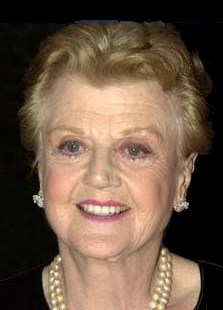
\includegraphics[width=\textwidth]{gandhi/from_57_1.png}
		\caption{оригинал}
	\end{subfigure}
	\begin{subfigure}[t]{0.25\textwidth}
		
\includegraphics[width=\textwidth]{gandhi/from_57_2.png}
		\caption{искривлённое изображение}
	\end{subfigure}
	\begin{subfigure}[t]{0.25\textwidth}
		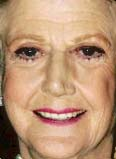
\includegraphics[width=\textwidth]{gandhi/from_57_3.png}
		\caption{с исправленной гистограммой}
	\end{subfigure}
	\caption{Коррекция изображений в методе Gandhi}
	\label{fig:gandhi}
\end{figure}

Затем оператор расставляет на изображении порядка двадцати ключевых точек, отмечая положение отдельных частей лица и на основе этих точек генерируются сплайны, подчеркивающие основные черты лица. Авторы статьи сознательно отказываются от алгоритмов автоматической разметки лица вроде ASM \cite{asm}, ссылаясь на низкое качество их работы на момент написания статьи (2004 год). После этого изображение искривляется (warp) с использованием собственного алгоритма для приведения координат отмеченных точек к координатам точек средней формы (см. рис. \ref{fig:gandhi} ).

Анализируя опыт и ошибки предшественников в автоматическом определении возраста, авторы статьи решили, что причина неудач кроется в малом количестве изображений в обучающей выборке и в низком их качестве, поэтому они собрали собственную базу изображений. Эта база состоит из 800 фотографий знаменитостей, сделанных профессиональными фотографами, отобранных вручную с целью исключить фотографии, где выражение лица далеко от нейтрального.

Для оценки возраста авторы статьи использовали метод опорных векторов, а точнее -- регрессию опорных векторов (SVR). Регрессия эта построена между числом, означающим возраст, и вектором, содержащим пиксели трансформированного изображения.

Параметры SVR, такие как вид ядра и его параметры, значение $ \varepsilon $ для чувствительности функции потерь, максимальная ошибка в критерии сходимости, были получены в результате экспериментов сперва грубо, затем с более высокой точностью с помощью кросс-валидации.

С помощью различных ухищрений, таких как переход в частотное пространство (т.е. использование в качестве входных векторов не само изображение, а его вейвлет-разложение), маскирование нелицевых областей, изменение размера изображения и т.д. удалось снизить минимальную абсолютную ошибку до 9 лет на всех возрастных группах и до 1-3 лет на отдельных образцах.

\subsubsection{Age and Gender Estimation of Unfiltered Faces}
Более современные подходы также используют модифицированный метод опорных векторов. Статья \cite{svm_dropout} вводит так называемый dropout-SVM, что позволяет им оценивать возраст изображений без ограничений по условиям съёмки. Алгоритм начинает работу с поиска лица алгоритмом Виолы-Джонса \cite{viola_jones}, затем производит выравнивание лица с использованием детектора ключевых точек, описанного в 2012 году Zhu and Ramanan \cite{zhu_ramanan}. Используя вместо самого изображения его представление с помощью локальных бинарных шаблонов \cite{lbp}, обучается обыкновенный линейный SVM-классификатор, однако интересна методика его обучения. Авторы, очевидно, были вдохновлены методом обучения искуственных нейронных сетей под названием dropout, когда в процессе обучения на отдельных итерациях временно выбрасывается какая-то доля (обычно 50\%) случайно выбранных нейронов, за счёт чего остальные нейроны лучше адаптируются к входным данным и меньше полагаются на работу соседних нейронов. А поскольку линейный SVM-классификатор реализует решающее правило, которое можно представить искуственной нейронной сетью с одним входным слоем и одним выходом, то можно провести аналогичную процедуру для входного слоя, на каждом этапе обучения случайным образом зануляя различные отдельные значения входного вектора. Полученный классификатор является гораздо более робастным (т.е. устойчивым к выбросам), чем линейный SVM, обученный традиционными методами, авторы оценивают увеличение точности минимум на 6\%.

В среднем, полученная система угадывает возрастную группу (разброс возрастов в каждой группе составляет 5-7 лет) в 67\% случаев на семейных фотографиях и почти 50\% на фотографиях из соцсетей \cite{adience}.

\subsubsection{Age and Gender Classification Using Convolutional Neural Networks}
Те же авторы буквально в мае текущего года выпустили ещё одну статью \cite{cnn_age_gender}, посвященную проблеме автоматической оценки возраста. На этот раз для оценки возраста и пола было предложено использовать свёрточные нейросети, находящиеся сегодня на очередном пике популярности. Архитектура нейросети, предложенная авторами, позволяет передать на вход отмасштабированное до $256 \times 256$ RGB-изображение лица, в произвольной позе и с произвольным выражением лица, и получить на выходе одну из возрастных категорий:
\begin{itemize}
\item от 0 до 2 лет
\item от 4 до 6 лет
\item от 8 до 12 лет
\item от 15 до 20 лет
\item от 25 до 32 лет
\item от 38 до 43 лет
\item от 48 до 53 лет
\item от 60 до 100 лет
\end{itemize}

Нейросеть состоит из трёх свёрточных слоёв (96 фильтров $7 \times 7$, 256 фильтров $5 \times 5$, 384 фильтров $3 \times 3$) и двух полносвязных, каждый по 512 нейронов (см. рис. \ref{fig:cnn}). На всех слоях в качестве активационной функции используется ReLU, один из вариантов которой выглядит так:

$$
f(x)={\begin{cases}x,&{\mbox{if }}x>0\\0.01x,&{\mbox{otherwise}}\end{cases}}
$$

Использование ReLU - довольно популярная практика в обучении нейросетей. Смысл использования ReLU состоит в добавлении нелинейности, что, по некоторым данным, даёт возможность приблизить с помощью нейросети практически любую функцию. Другим важным свойством ReLU является то, что её градиент либо равен единице, либо очень близок к нулю, и, следовательно, не может произойти разрастание или затухание градиентов при обучении нейросети методом обратного распространения ошибки.

\begin{figure}[t]
	\centering
	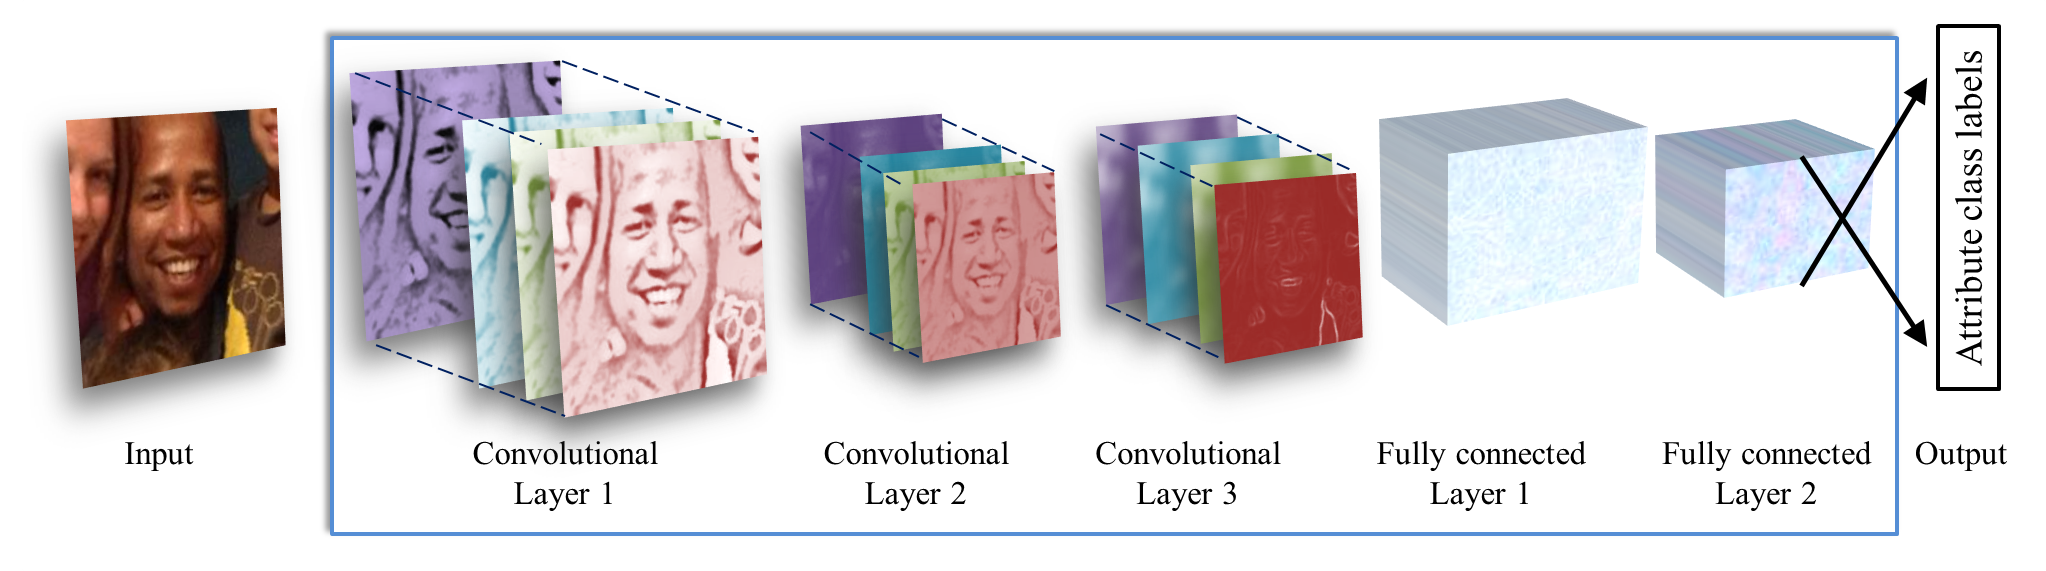
\includegraphics[width=\textwidth]{cnn.png}
	\caption{Архитектура нейросети для определения возраста}
	\label{fig:cnn}
\end{figure}

Авторы отмечают, что относительно малое число слоёв было использовано с целью избавиться от переобучения, столь характерного для других популярных алгоритмов определения возраста. Что интересно, авторы используют такую же архитектуру нейронных сетей для определения пола, но в качестве выходного слоя используется всего два выхода.

К достоинствам описанного подхода можно отнести простоту реализации. Для определения возрастной группы человека достаточно простейшей предобработки изображения (кадрирование лица и масштабирование до размера, принимаемого нейросетью), после этого для оценки возраста достаточно будет воспользоваться обученными весами нейросети и произвести один прямой проход по сети, что можно сделать с помощью любого фреймворка для работы с нейросетями.

Недостатки у этого подхода в целом такие же, как и у всех методов, использующих нейросети, однако, связаны они не с качеством работы метода, а с недостаточно проработанной теорией нейросетей. Так, выбор архитектуры сети ничем не обусловлен; метод в явном виде не производит нормализацию изображения, поиск ключевых точек и остальные необходимые операции из <<конвееров>> по оценке возраста. Исследователи полностью полагаются на нейросеть, в надежде, что все эти операции в неявном виде будут реализованы на различных её уровнях. Это означает, что если на некоторых наборах входных данных результаты будут неудовлетворительными, останется лишь гадать, почему. Кроме того, исследователи не учитывают процесс старения лица вообще, в частности, определение возраста происходит по неупорядоченным группам. Поэтому они, однако, с такой лёгкостью адаптировали нейросеть всего к двум кластерам для определения пола, исходя, видимо, из соображения, что внешность людей разных возрастов с точки зрения компьютера отличается так же сильно, как и внешность людей разных полов.

Однако, цель работы - рассмотреть наиболее предпочтительные подходы с практической, а не с теоретической точки зрения. И если производительность этого подхода окажется выше, чем у конкурирующих, это достоинство перевесит все перечисленные недостатки.

\subsection{Эксперименты с оценкой возраста}

Для оценки производительности был выбран последний из описанных методов, использующий искусственные нейросети. Главной причиной тому является то, что авторы выложили обученную ими нейросеть, что даёт нам возможность не задумываться о неочевидных деталях, которые мы могли бы упустить при самостоятельной реализации метода, а сосредоточиться на практической проверке его качества. Что касается остальных методов оценки возраста, то методы 2004 года и ранее предъявляют очень высокие требования к качеству входных изображений и сопутствующих данных. Так, метод из статьи Gandhi \cite{statya_big} обязательно требует изображений в хорошем разрешении, снятых в закрытом помещении с равномерным светом, не говоря уже о том, что он требует от пользователя вручную расставить на изображении ключевые точки. Несмотря на то, что с 2004 года появилось несколько детекторов ключевых точек с гораздо более высокой точностью, чем популярные в то время, такие как детекторы от Jason Saragih \cite{jsaragih} или от Zhu и Ramanan \cite{zhu_ramanan}, требование расставлять точки вручную означает практически абсолютную точность, без которой корректная работа алгоритма не может быть гарантирована. Авторы же подхода с использованием нейросетей заявляют, что их метод устойчив к плохим условиям съёмки.

Для оценки производительности данного метода был использован набор изображений Adience Benchmark \cite{adience}. Изображения в данном датасете были собраны из социальной сети Flickr и снабжены подробными описаниями, включающими в себя индивидуальный номер, закреплённый за каждым человеком с фотографий, пол, возрастную группу (с разбросом в 5-7 лет), а также некоторые данные о геометрии лица, включая описывающй лицо прямоугольник и оценённые автоматически углы поворота головы в трёхмерном пространстве. Пользуясь этой информацией, изображения были подвергнуты афинным преобразованиям с целью выровнять лица до пропорций, близких к пропорциям лиц анфас. База данных содержит порядка 20000 изображений, снятых преимущественно любителями на камеры смартфонов, в базе большое количество совместных фотографий, сэлфи, фотографий с посторонними объектами, с низкой четкостью и неровным освещением.

Такой набор данных позволит выяснить, насколько алгоритм устойчив к помехам, искажениям и плохим условиям съёмки. Более того, можно будет выяснить, насколько сильно зависит результат работы алгоритма от условий съёмки, отобрав фотографии с различным качеством и проследив за тем, возникают ли ошибки определения возраста чаще на низкокачественных фотографиях.

Из всех изображений базы были случайно выбраны 3210 изображений. Из базы были исключены изображения, для которых не указан возраст или указанный возраст находится вне возрастных рамок, которые способен был бы определить алгоритм. Остальные изображения были пропущены через обученную авторами работы нейросеть, после чего было проведено сравнение реального возраста с оценённым. Для тестирования был использован фреймворк для работы с искусственными нейросетями Caffe и Numpy для загрузки изображений и их подготовке для нейросети.

Оценка качества алгоритма производилась с учётом того, что он на самом деле решает не задачу регрессии между возрастом и характеристиками изображения, а задачу классификации изображения как принадлежащего одному из классов. Поэтому было оценено не только число лет, на которое ошибся алгоритм, но и ошибка в определении возрастной группы. Во внимание были также приняты результаты, полученные авторами статьи.

Результаты приведены в таблице \ref{table:age_precision}. Они в среднем на 3\% ниже, чем результаты, приведённые авторами статьи, что можно объяснить меньшей выборкой для тестирования.

\newcolumntype{d}[1]{D{,}{,}{#1} }
\makeatletter
\newcolumntype{B}[3]{>{\boldmath\DC@{#1}{#2}{#3} }c<{\DC@end} }
\newcolumntype{Z}[3]{>{\mathversion{nxbold}\DC@{#1}{#2}{#3} }c<{\DC@end} }
\makeatother

\begin{table}
\caption{Точность детектирования возраста}
\small
{
\begin{tabular}{|l|d{2}|d{2}|d{2}|d{2}|r|}
\hline
Возраст & 
\multicolumn{1}{c|}{ \parbox[t]{2.35cm}{ верно \\ угаданных, \%} }  & 
\multicolumn{1}{c|}{ \parbox[t]{2.35cm}{ Средняя \\ ошибка, лет } } & 
\multicolumn{1}{c|}{ \parbox[t]{2.35cm}{ Средняя \\ абсолютная \\ ошибка, лет } } &
\multicolumn{1}{c|}{ \parbox[t]{2.35cm}{ Стандартное \\ отклонение, лет } } & 
\parbox[t]{2cm}{ Общее \\ кол-во } \\
\hline
\enspace 0 - 2   & 65,03 &   2,77 &  2,77 &  6,32 &  675 \\
\enspace 4 - 6   & 33,97 &   2,70 &  5,26 &  8,93 &  365 \\
\enspace 8 - 12  & 60,00 &   4,54 &  6,76 & 12,03 &  160 \\
        15 - 20  &  0,00 &   8,69 & 12,39 & 10,88 &  111 \\ 
        25 - 32  & 58,96 &  -4,04 &  7,74 & 12,08 & 1143 \\
        38 - 43  & 20,29 & -14,36 & 14,55 & 12,19 &  404 \\
        48 - 53  &  0,02 & -23,74 & 23,74 & 13,55 &  167 \\
        60 - 100 &  0,06 & -45,70 & 45,70 & 18,08 &   94 \\
\hline
Всего &  45,69 &  -4,39 &  9,37 & 14,72 & 3121 \\
\hline
\end{tabular}
}
\label{table:age_precision}
\end{table}

В первую очередь нужно заметить, что несмотря на результат в 45\% угадывания возрастной категории, средняя ошибка в определении возраста составляет чуть более девяти лет, как и в старом алгоритме из статьи Gandhi \cite{statya_big}. Кроме того, возможно, набор обучающих изображений для нейросети не был сбалансирован, поскольку лишь на двух категориях изображений достигается результат около 60\% и выше (от 0 до 2 лет и от 25 до 32 лет), за счёт них нейросеть и имеет такой относительно высокий средний результат детектирования.

\begin{table}
\caption{Результаты классификации возраста, \%}
\normalsize 
{
\begin{tabular}{|l|d{1} d{1} d{1} d{1} d{1} d{1} d{1} d{1}|d{1}|}
\hline
Возраст &
\multicolumn{1}{c}{0-2}   &
\multicolumn{1}{c}{4-6}   &
\multicolumn{1}{c}{8-12}  &
\multicolumn{1}{c}{15-20} &
\multicolumn{1}{c}{25-32} &
\multicolumn{1}{c}{38-43} &
\multicolumn{1}{c}{48-53} &
\multicolumn{1}{c|}{60-100}&
\multicolumn{1}{c|}{Доля} \\
\hline
\enspace 0 - 2   & \multicolumn{1}{Z{,}{,}{1}}{65,0} & 23,9 &  7,4  &  0,0 &    2,8 &  0,6 &   0,3 &  0,0 & 21,6 \\
\hline
\enspace 4 - 6   & 32,0 & \multicolumn{1}{Z{,}{,}{1}}{33,9} & 23,2  &  0,0 &    9,0 &  1,6 &   0,3 &  0,0 & 11,7 \\
\hline
\enspace 8 - 12  &  6,8 &    9,9 & \multicolumn{1}{Z{,}{,}{1}}{59,6}&  0,0 &   14,9 &  8,1 &   0,0 &  0,6 &  5,2 \\
\hline
        15 - 20  &  4,5 &    1,8 & 11,7 & \multicolumn{1}{Z{,}{,}{1}}{0,0} &   73,0 &  7,2 &   0,9 &  0,9 &  3,6 \\
\hline
        25 - 32  &  8,0 &    3,9 & 14,9 &  0,3  & \multicolumn{1}{Z{,}{,}{1}}{59,0} & 13,0 &   0,7 &  0,3 & 36,6 \\
\hline
        38 - 43  &  9,7 &    2,2 &  9,9 &  0,2  & 56,4 & \multicolumn{1}{Z{,}{,}{1}}{20,5} &   1,0 &  0,0 & 12,9 \\
\hline
        48 - 53  & 13,8 &    2,4 &  5,4 &  0,0  & 50,9 &   24,6 & \multicolumn{1}{Z{,}{,}{1}}{3,0} &  0,0 &  5,4 \\
\hline
        60 - 100 &  8,5 &    2,1 &  6,4 &  0,0  & 26,6 &   44,7 &  5,3 & \multicolumn{1}{Z{,}{,}{1}|}{6,4} &  3,0 \\
\hline
 ~~     Все      & 18,5 &   10,0 & 17,3 &  0,1  & 36,6 &   15,0 &  1,4 &   1,0 & 100,0 \\
\hline
\end{tabular}
}
\label{table:age_confusion}
\end{table}

В таблице \ref{table:age_confusion} представлено распределение результатов классификации внутри каждого кластера: для каждого фиксированного реального возраста в строке указана условная вероятность детектирования каждого кластера из столбца.


На всех группах изображений дисперсия ошибки больше, чем разброс внутри группы, что говорит о том, что б$ \grave{o} $льшая часть ошибок в детектировании пришлась на соседние группы. Действительно, реальная возрастная группа отличается от предсказанной не более чем на один соседний кластер в 75\% случаев. Эти результаты подтверждаются авторами статьи, которые пишут о 80\% угадывании с ошибкой в один кластер.

Анализ ошибочных изображений подтвердил некоторые выводы, сделанные ранее. Так, если на изображении - женщина, это увеличивает вероятность ошибки, причём в отрицательную сторону. Отчасти это связано с использованием макияжа. Однако более вероятно, что дело здесь в том, что нейросеть обучалась одновременно и на мужчинах, и на женщинах. Процесс старения же у мужчин и женщин отличается, как правило мужские лица с возрастом меняются значительно быстрее. В результате лица с меньшими возрастными изменениями воспринимаются нейросетью как более молодые.

А вот нетребовательность алгоритма к условиям съёмки была подтверждена. В процессе анализа ошибочных изображений не было выявлено зависимости между качеством фотоснимка и размером ошибки. Среди верно классифицированных изображений присутствовали как изображения в хорошем качестве с ровным освещением, так и низкокачественные фотографии с размытыми деталями, неровным светом и экстремальными выражениями лица.
